\chapter{The Arrow, the Hours, and the Cliff}

In this School of Hard Knocks interview, curated by LazyingArt LLC, Will Smith gives us a sequence that is much more structured than the surface glamour suggests. The published video first throws out its hooks in teaser form: bad advice, money and misery, giant years, and celebrity scale. The actual conversation then fills in the mechanism underneath the hooks. We are led from mastery to diversification, from hours to cumulative advantage, from suffering to enlargement, from failure to confidence, from relationships to money, and finally to a harder claim: material success has its own abyss, and the real search beneath both poverty and abundance is for steadiness in the self.

\section{Opening Shock, Then the Actual Entrance}

The lecture begins twice. First we are given the condensed future version: a few sharp claims, almost as if the result is known before the proof. Then the video restarts in ordinary time. There is a gate, a walk-up, a greeting, some easy talk, names, and the immediate human reduction of celebrity scale into conversational distance. That duplicated opening should be kept, because the lecture wants to stage magnitude before it explains mechanism.

The first substantive fact is simple and negative:
\[
\text{starting capital} \approx 0,
\qquad
\text{family money} = 0
\]
in the blunt sense in which Smith says he came from ``the opposite'' of money. The point is not numerical bookkeeping. The point is that later claims about freedom, craft, and judgment are not introduced as the inheritance of ease.

What follows is not yet theory. It is the setup for theory. We are told who is here, and then we are told what he has done: music, television, film, production, business. The plurality of roles creates the first real problem of the chapter. If the career is this spread out, why does the lecture soon insist so strongly on one-point mastery?

\section{Many Hyphens, One Arrow}

Smith's career description produces an immediate tension. On the surface, he appears to be an argument for diversification. He is not one thing. He is many things. The host sees that at once and asks the correct question: should a young person focus on one thing, or distribute effort across multiple ventures?

Smith's answer is the lecture's first decisive construction. He says to think of it like an arrow. The tip must be sharp, singular, and precise. Only after the arrow has broken through do the other things come through behind it. In companion-note form we can write the lecture's logic as
\begin{equation}
\text{mastery}(x_{\mathrm{tip}})
\Longrightarrow
\text{expansion}(\mathcal D_{\mathrm{trail}}),
\end{equation}
where \(x_{\mathrm{tip}}\) is the one thing done ``really specifically and really well,'' and \(\mathcal D_{\mathrm{trail}}\) is the family of later domains that are allowed to follow.

\begin{figure}[h]
\centering
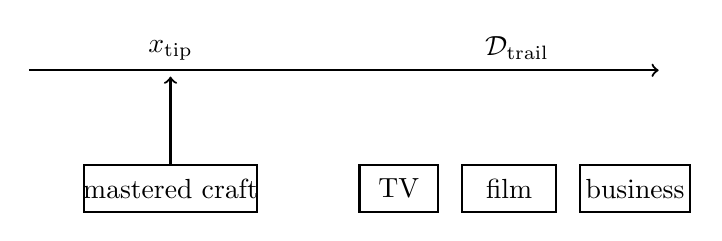
\begin{tikzpicture}[x=1cm,y=1cm,thick]
\draw[->] (0,0) -- (8,0);
\node[above] at (1.8,0) {$x_{\mathrm{tip}}$};
\node[above] at (6.2,0) {$\mathcal D_{\mathrm{trail}}$};

\draw (0.7,-1.2) rectangle (2.9,-1.8);
\node at (1.8,-1.5) {mastered craft};
\draw[->] (1.8,-1.2) -- (1.8,-0.08);

\draw (4.2,-1.2) rectangle (5.2,-1.8);
\node at (4.7,-1.5) {TV};

\draw (5.5,-1.2) rectangle (6.7,-1.8);
\node at (6.1,-1.5) {film};

\draw (7.0,-1.2) rectangle (8.4,-1.8);
\node at (7.7,-1.5) {business};
\end{tikzpicture}
\caption{Transcript-derived arrow schematic. The point is not that one must remain in one domain forever. The point is that later domains are most durable when they are pulled behind a real point of penetration.}
\end{figure}

The lecture strengthens the same thought with the image from \emph{The Alchemist}: the whole universe is contained in a grain of sand. In the present context, that is not mystical ornament. It is an epistemic rule. If we understand one thing deeply enough, that one thing becomes an instrument for understanding adjacent things. Local mastery is not local forever.

\subsection{Question \& Answer}

\paragraph{Question.} Should we diversify early, or master one thing first?

\paragraph{Answer.} Smith's answer is sequential rather than ideological. He is not against later plurality. He is against premature plurality. The lecture's order is
\[
\text{point first}, \qquad \text{trail later}.
\]
This is why the arrow matters. A dull object with many attachments is not the same thing as a sharp object with a disciplined direction.

\section{The Arithmetic of Hours}

Once the arrow has been established, the lecture asks a harder question. Even if we accept focus before spread, what actually separates the person who breaks through from the person who almost does?

Smith answers with time. He says the wind goes to the most hours committed. That is a compact statement, but it contains the chapter's clearest arithmetic. Let \(h\) denote hours committed per day and let \(H(T)\) denote cumulative committed hours over \(T\) days. Then the lecture's simple counting model is
\begin{equation}
H(T)=h\,T.
\end{equation}
Now compare two operators:
\begin{equation}
H_A(365)=10\cdot 365,
\qquad
H_B(365)=9\cdot 365.
\end{equation}
The gap after one year is then
\begin{align}
\Delta H
&=H_A(365)-H_B(365) \\
&=(10-9)\cdot 365 \\
&=365\ \text{hours}.
\end{align}

This is the chapter's cleanest worked derivation because it makes Smith's point precise without pretending that he is giving us a theorem of destiny. A one-hour edge sounds trivial at the scale of one afternoon. It is not trivial at the scale of a year.

We can sharpen the same comparison by looking at the ratio:
\begin{equation}
\frac{H_A(365)}{H_B(365)}=\frac{10}{9}\approx 1.11.
\end{equation}
So the lecture is really saying that a steady one-hour daily advantage yields about an eleven-percent cumulative edge in committed time over a year. We do not need to claim more than that. Smith's own conclusion is qualitative: if the time gap is real and sustained, even talent may have trouble overcoming it.

\paragraph{Mechanism.}
This section matters because it prevents the lecture from dissolving into vague ambition. The arrow gave us direction. The hours give us propulsion. The lecture is not saying that all outcomes reduce to labor. It is saying that visible superiority often conceals a long arithmetic of attention.

\section{The Small Person, Suffering, and the Larger Energy}

The lecture now widens from career strategy to a view of the self. As an actor, Smith says that what we call a person is not really the whole person. It is more like a personality, a small constellation of ideas chosen and inhabited. In companion-note notation we may write, cautiously,
\begin{equation}
P \subsetneq \mathcal S,
\end{equation}
where \(P\) is the narrow personality-construct and \(\mathcal S\) the larger self that exceeds the sliver of race, city, creed, history, and habit to which we ordinarily confine ourselves.

That move is immediately followed by adversity. In the discussion of Chris Gardner and the film about him, suffering is not treated as accidental damage. It is treated as education. Difficulty shapes willpower, energy, and endurance. In compressed form the lecture's logic is
\begin{equation}
\text{difficulty}
\longrightarrow
\text{shaping of willpower}
\longrightarrow
\text{greater usable force}.
\end{equation}
This is why the line about getting comfortable being uncomfortable belongs here. The point is not merely stoicism. The point is formation.

Faith then enters without breaking the argument. Smith says he believes in a creative energy at work in all things and that relation to it enlarges his power beyond the ego's ordinary limits. The safest way to preserve that claim is not to over-formalize it. We can simply keep its asymmetry:
\begin{equation}
\text{creative capacity}_{\mathrm{ego}}
<
\text{creative capacity}_{\mathrm{aligned}}.
\end{equation}
He uses ``a hundredfold'' as the language of enlargement. In these notes we should keep that as rhetorical scale, not as a measurable multiplier.

The important structural point is that the lecture refuses to leave success at the level of technique. Mastery in the public world is tied back to the size of the self that does the mastering. If the self is small, brittle, and overidentified with the mask, then the public machine can only go so far.

\section{Confidence After the Miss}

The next problem is introduced perfectly. If the world rewards the courageous and if confidence seems to matter so much, where does confidence actually come from? Smith's answer is that it does not begin as the polished social state we later call confidence. It begins as the willingness to look stupid.

This is one of the lecture's best reversals. What we perceive as confidence is often just repeated survival in public after visible failure. Smith makes the point with comedy and performance rather than with statistics, but he gives us one useful ratio:
\begin{equation}
p_{\text{hit}}=\frac{3}{10}=0.3.
\end{equation}
The point is not that \(30\%\) is a universal benchmark. The point is that public excellence does not require the fantasy of perfect execution. If three good outcomes out of ten place one ``in the hall of fame,'' then missing is not evidence against the path. Missing is part of the path.

\paragraph{Anecdote.}
The lecture ties this to \emph{The Fresh Prince of Bel-Air}. Confidence is one side of what we see. The underlying substrate is different: not being destroyed by the fear of doing it wrong in front of other people.

\paragraph{Claim.}
Confidence is not an initial possession. It is a later appearance.

\paragraph{Mechanism.}
The process is
\[
\text{visible attempt}
\to
\text{miss}
\to
\text{survival}
\to
\text{repetition}
\to
\text{reduced fear}
\to
\text{perceived confidence}.
\]
The lecture's phrasing is more human than formal, and that is exactly right. We are not deriving a psychological law. We are preserving a practical sequence.

\subsection{Question \& Answer}

\paragraph{Question.} What is confidence actually made of?

\paragraph{Answer.} In this lecture, it is made of tolerated embarrassment. The host asks about belief and success; Smith answers with something more primitive and more exact. Confidence is what other people call the person who is no longer paralyzed by the cost of looking foolish. It is therefore built not before failure, but after enough failure has stopped having veto power.

\section{Advice, Intuition, and the Network of the Future}

Once the lecture has explained how confidence is built, it turns to the problem of guidance. Here Smith returns to one of the cold-open claims and gives it its full moral weight. Taking advice from somebody who has not done what we want to do is, in his language, almost insanity.

We can render that filter schematically as
\begin{equation}
\mathcal A_{\mathrm{admissible}}
=
\{x:\ x \text{ has actually done the thing in question}\}.
\end{equation}
Again, the point is not set theory for its own sake. It is the discipline of shrinking the class of voices we permit to shape a trajectory.

The Quincy Jones story sharpens the argument. Smith asks for advice; Quincy declines to counterfeit certainty about a life he himself would not have chosen. That refusal becomes one of the lecture's strongest indirect lessons. Serious people do not always answer. Sometimes they recognize the limit of transfer.

From here the lecture moves from explicit advice to behavior-reading. Ask for advice less. Watch more. Listen more. Let conduct tell us what a person really thinks. That path ends, naturally, in the bird-and-branch analogy:
\begin{equation}
\text{trust}(\text{wings}) > \text{trust}(\text{branch}).
\end{equation}
This is not a literal inequality from the speaker. It is a faithful schematic translation of the image. The branch may be weak or strong; the bird survives because it carries the means of re-stabilization within itself.

At this point the published lecture breaks for a long promotional interruption. When it returns, it returns to mentors and to the social field rather than to money first. Smith remembers his grandmother's warning: everywhere we go, one day we may have to go back. That becomes a theory of delayed human value. The lecture's timeline is explicit enough to preserve:
\begin{equation}
16
\Longrightarrow
24
\Longrightarrow
34.
\end{equation}
Someone we meet now may later be running the company we want to sell to. Later still, the relationship may reappear through family, school, or some other institutional crossing.

This is the right place to add a second correction about craft and success. The host loops back, after this social doctrine, to the turning point of financial freedom. Smith says something extremely exact: what we like is not always what we are best at.
\begin{equation}
\text{preference} \neq \text{comparative advantage}.
\end{equation}
He loved music. He says he was better as an actor. The turning point was not mere hustle. It was choosing the stronger craft and allowing finance to arrive behind mastery rather than in front of it.

\section{Money, the Threshold, and the Clifftop}

The lecture now returns to money directly. Smith avoids naming the largest dollar figure, but he does name a peak creative-financial interval: \emph{Hancock} and \emph{I Am Legend} landing within roughly six months of each other. The point is not bragging. It is that large years are still meaningful to him primarily as creative periods, not only as cash periods.

Then the lecture tightens into its hardest scalar claim. Money does not buy happiness. More than that, past some level it begins to buy misery. Smith gives a rough threshold, clearly as heuristic rather than law:
\begin{equation}
m_\ast \approx \$1{,}000{,}000/\text{year}.
\end{equation}
The chapter should preserve the claim in that spirit:
\begin{align}
m \lesssim m_\ast
&\Rightarrow
\text{money removes real constraints},\\
m \gtrsim m_\ast
&\Rightarrow
\text{money may begin to add suspicion, distortion, and attack.}
\end{align}
The lecture's wording is social before it is psychological. At certain financial levels, making new friendships becomes difficult. People think about the money. Social interpretation bends. The person enters what Smith calls an attack zone.

Now the host introduces the chapter's most important late image: clifftop versus rock bottom. Everybody thinks the changing moment comes at the bottom. Smith says there is a corresponding upper abyss. After enough money, sex, fame, and acquisition, one can arrive at a different form of emptiness. Nothing left to buy. Nobody new to pursue. Nothing material that still promises satisfaction.

We may write the symmetry schematically as
\begin{equation}
\mathcal A_{\mathrm{rock\ bottom}}
\sim
\mathcal A_{\mathrm{clifftop}}.
\end{equation}
This is not a rigorous equivalence. It is a transcript-faithful symmetry claim. Both abysses expose the same inadequacy of material solutions.

\begin{figure}[h]
\centering
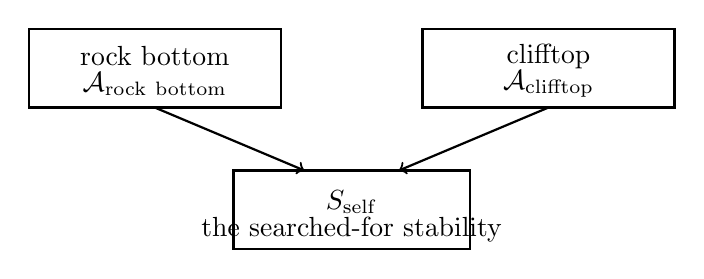
\begin{tikzpicture}[x=1cm,y=1cm,thick]
\draw (0,0) rectangle (3.2,1);
\node at (1.6,0.65) {rock bottom};
\node at (1.6,0.3) {$\mathcal A_{\mathrm{rock\ bottom}}$};

\draw (5.0,0) rectangle (8.2,1);
\node at (6.6,0.65) {clifftop};
\node at (6.6,0.3) {$\mathcal A_{\mathrm{clifftop}}$};

\draw (2.6,-1.8) rectangle (5.6,-0.8);
\node at (4.1,-1.2) {$S_{\mathrm{self}}$};
\node at (4.1,-1.55) {the searched-for stability};

\draw[->] (1.6,0) -- (3.5,-0.8);
\draw[->] (6.6,0) -- (4.7,-0.8);
\end{tikzpicture}
\caption{Transcript-derived symmetry of the two abysses. Deprivation and saturation are not the same social condition, but they can reveal the same inner instability.}
\end{figure}

Smith's resolution is blunt. What we are actually looking for is ourselves. The real object is a steadiness that can survive weak branches, failed relationships, incurable illness, and death. This is why the bird-and-branch analogy returns here with greater force. If the branch is our material condition, then no branch is safe enough. Safety comes from becoming trustworthy to ourselves.

\subsection{Question \& Answer}

\paragraph{Question.} Why can success become its own kind of cliff?

\paragraph{Answer.} Because material abundance can complete the material program without answering the deeper question. Rock bottom tells us that we do not have enough. Clifftop tells us that enough was never the same thing as peace. The lecture insists that both discoveries are painful, and that both point past possession toward self-stability.

The closing exhortation to the younger generation follows directly from this. Consciousness, Smith says, is a crazy gift that can do almost anything. One need not keep the job, the town, or the current relational form. But the price of exercising that freedom is not fantasy. It is suffering. That is the final correction with which the lecture ends. Infinite seeming possibility still meets cost.

\section{Summary}

The chapter begins with scale and ends with self. In between, it builds a strict sequence. We sharpen one point before we spread into many domains. We accumulate hours before we claim superiority. We allow suffering to shape force rather than only injure it. We stop pretending confidence is effortless and admit that it is built from public misses. We filter advice by proof, then move from proof toward intuition. We treat relationships as long-horizon structure rather than as accidental encounters. And finally we recognize that money can remove constraints without solving the deeper problem of who is living inside the machine.

That is why the last architecture of the lecture matters so much. The arrow and the hours explain how one rises. The cliff explains what rising still cannot solve.